%%% License: Creative Commons Attribution Share Alike 4.0 (see https://creativecommons.org/licenses/by-sa/4.0/)
%%% Slides are based heavily on earlier versions of this course taught by Jesper Rudiger.

\documentclass[english,10pt
%,handout
,aspectratio=169
]{beamer}
%%% License: Creative Commons Attribution Share Alike 4.0 (see https://creativecommons.org/licenses/by-sa/4.0/)
%%% Slides are based heavily on earlier versions of this course taught by Jesper Rudiger and Peter Norman Sorensen.

\DeclareGraphicsExtensions{.eps, .pdf,.png,.jpg,.mps,}
\usetheme{reMedian}
\usepackage{parskip}
\makeatother

\renewcommand{\baselinestretch}{1.1} 

\usepackage{amsmath, amssymb, amsfonts, amsthm}
\usepackage{enumerate}
\usepackage{hyperref}
\usepackage{url}
\usepackage{bbm}
\usepackage{color}

\usepackage{tikz}
\usepackage{tikzscale}
\newcommand*\circled[1]{\tikz[baseline=(char.base)]{
		\node[shape=circle,draw, inner sep=-20pt] (char) {#1};}}
\usetikzlibrary{automata,positioning}
\usetikzlibrary{decorations.pathreplacing}
\usepackage{pgfplots}
\usepgfplotslibrary{fillbetween}
\usepackage{graphicx}

\usepackage{setspace}
%\thinmuskip=1mu
%\medmuskip=1mu 
%\thickmuskip=1mu 


\usecolortheme{default}
\usepackage{verbatim}
\usepackage[normalem]{ulem}

\usepackage{apptools}
\AtAppendix{
	\setbeamertemplate{frame numbering}[none]
}
\usepackage{natbib}




\title{Financial Markets Microstructure \\ Lecture 8}

\subtitle{Empirics of illiquidity\\
	Chapter 5 of FPR}

\author{Egor Starkov}

\date{K{\o}benhavns Unversitet \\
	Spring 2021}


\begin{document}
	
\AtBeginSection[]{
	\frame<beamer>{
		\frametitle{This lecture:}
		\tableofcontents[currentsection,currentsubsection]
}}

\frame[plain]{\titlepage}

%\section{Revision and problems}

\begin{frame}{What did we do last week?}
	\begin{enumerate}
		\item The spread is not only driven by adverse selection: order costs and inventory risk have an effect as well
		\item However, we would expect the dynamic effect of these three different mechanisms to be different
		\begin{itemize}
			\item Order costs: only short-run effect 
			\item Inventory risk: medium-run effect, but should be zero in the long run
			\item Adverse selection: long-run effect 
		\end{itemize}
	\end{enumerate}
\end{frame}


\begin{frame}{Today}
	\begin{itemize}
		\item \textbf{Empirical estimation}
		\begin{itemize}
			\item Before we looked at how to estimate the spread, but without a theory for what drives it
			\item Thus: talk about estimating drivers of the spread
			\item Furthermore:
			\begin{itemize}
				\item Look at estimating price impact/depth
				\item Look at estimating proportion of informed trading
			\end{itemize}
		\end{itemize}
	\end{itemize}
\end{frame}



\section{Empirics of illiquidity}

\begin{frame}{Introduction}
	\begin{itemize}
		\item What determines illiquidity?
		\begin{itemize}
			\item Chapter 2 discussed empirical measures of illiquidity
			\item Chapters 3 and 4 developed some theories
			\item Can we detect the relative importance of theoretical effects on the measures?
		\end{itemize}
		\item The end of chapter 3 discussed the various price impacts of transaction costs, informed trading, market maker risk aversion (figure 3.9)
		\begin{itemize}
			\item Chapter 4: greater price change when transaction is larger
		\end{itemize}
	\end{itemize}
\end{frame}


\begin{frame}{}
	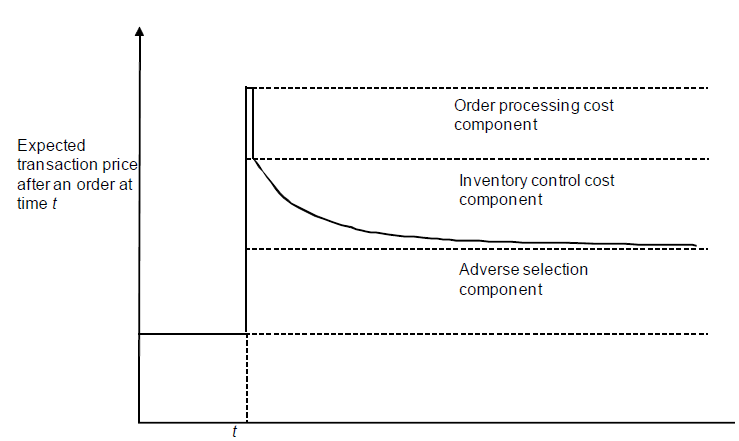
\includegraphics[width=0.8\linewidth]{pics/PriceDiscovery_Image}
\end{frame}


\begin{frame}{Measured price impact and the theories}
	\begin{itemize}
		\item Parameters of interest:
		\begin{itemize}
			\item $\gamma$: order-processing cost
			\item $\lambda$: price impact related to information
			\item $\beta$: price impact related to MM risk aversion
		\end{itemize}
		\item Data:
		\begin{itemize}
			\item Transaction prices $p_t$, net market order flow $q_t$, order sign $d_t$
		\end{itemize}
	\end{itemize}
\end{frame}


\begin{frame}{How to estimate?}
	\begin{itemize}
		\item Take GM model with order costs. There have:
		\begin{align*}
			p_t &= \mu_t + \gamma d_t
			\\
			\Rightarrow \varDelta p_t &= \mu_t - \mu_{t-1} + \gamma \varDelta d_t
		\end{align*}
		\item Further,
		\begin{align*}
			\mu_t = \mu_{t-1} + \lambda d_t + \varepsilon_t
		\end{align*}
		order flow is informative; also let $\varepsilon_t$ include all other kinds of public news
		\item Then
		\begin{align*}
			\varDelta p_t &= \lambda d_t + \gamma \varDelta d_t + \varepsilon_t
		\end{align*}
	\end{itemize}
\end{frame}


\begin{frame}{\cite{glosten_estimating_1988}}
	\begin{itemize}
		\item \textbf{\cite{glosten_estimating_1988}} estimate
		\begin{equation} \tag{5.7}
			\Delta p_t = \gamma_0 \Delta d_t+ \gamma_1 \Delta q_t + \lambda_0 d_t + \lambda_1 q_t + \epsilon_t
		\end{equation}
		jointly with trade directions $d_t$. 
		\item Accumulated order flow affects price level via $\lambda$, cyclical order flow gives $\gamma$ in the style of Roll's measure (2.15)
		\item On NYSE data from early 80s, they find $\gamma_1=\lambda_0=0$ and estimate $\gamma_0=.0465$, $\lambda_1=.0102$
	\end{itemize}
\end{frame}


\begin{frame}{Issues}
	\begin{itemize}
		\item Apart from the usual concerns with old empirical papers...
		\begin{itemize}
			\item not much data
			\item questionable specification
			\item questionable estimation procedures
		\end{itemize}
		\item ...there is the issue of ignoring inventory costs.
		\item In the short run, the effect of MM risk aversion would be similar
		\begin{equation} \tag{5.14}
		\Delta p_t = \gamma \Delta d_t + (\lambda + \beta) q_t + \epsilon_t
		\end{equation}
		\begin{itemize}
			\item $\lambda$ and $\beta$ are not separately identified.
		\end{itemize}
	\end{itemize}
\end{frame}


\begin{frame}[label=extending]{Including inventory costs}
	\begin{itemize}
		\item \textbf{\cite{hasbrouck_trades_1988}}: order flow is auto-correlated, so part of the order is not `news' but only moves inventory
		\item \textbf{\cite{huang_components_1997}}: suggest
		\begin{equation}\tag{5.17}
		q_t = \phi q_{t-1} + \eta_t
		\end{equation}
		\item Then (5.14) is modified to \hyperlink{derivation}{\beamerbutton{Derivation}}
		\begin{equation} \tag{5.21}
		\Delta p_t = \gamma \Delta d_t + (\lambda+\beta)q_t - \lambda \phi q_{t-1} + \epsilon_t
		\end{equation}
		\item They estimate the model for 20 major NYSE stocks: 
		\begin{align*}
			\phi &= -0.74	& \lambda &= 9.59\% S
			\\
			\beta &= 28.65\% S	& \gamma &= 61.76\% S
		\end{align*}
		%NOTE: negative phi makes sense with inventory costs
		\item Also: greater $\beta$ for larger transactions
	\end{itemize}
\end{frame}


\begin{frame}{Including inventory costs (2)}
		\begin{itemize}
			\item \textbf{\citet*{madhavan_why_1997}} find that $\lambda$ is higher in the morning, and $\gamma$ higher in the afternoon
			% more adverse selection in the morning; higher bargaining power for dealers at closing (traders want to unwind positions)
			\begin{itemize}
				\item Morning trading reveals all the information accumulated during off-market hours. Evening trading driven by traders' desire to close open positions
				\item \textbf{\cite{bogousslavsky_should_2020}}: closing auctions account for $7.3\%$ of daily trading volume, but contribute nothing to price discovery. Closing prices deviate a lot from midquotes, but revert back quickly.
			\end{itemize}
			\item \textbf{\cite{lyons_tests_1995}} had data on a FOREX dealer's inventory, and found $\beta$ very large
		\end{itemize}
\end{frame}


\begin{frame}{Long-run impact}
	\begin{itemize}
		\item Different dynamic approach: \textbf{\cite{hasbrouck_measuring_1991}} uses the long-run impact of an order $q_{t+1}$ on prices $p_{t+T}-p_t$ to identify the informational part of the trade
		\begin{itemize}
			\item The `impulse response' of prices to orders
			\item Opens door to richer time series analysis of transactions data
		\end{itemize}
		\item Findings: short-run effect of a trade $\approx 2\%$
		\item long-run effect of a trade ($T=5$ trades) $\approx 1\%$
		\begin{itemize}
			\item greater LR impact for stocks with lower capitalization
		\end{itemize}
	\end{itemize}
\end{frame}


\begin{frame}{Probability of Informed Trading}
	\begin{itemize}
		\item \textbf{\citet*{easley_liquidity_1996}}: use GM type model to estimate the prob. of informed trading
		\item On any given trading day, w.p. $\alpha$ there is some information event
		\begin{itemize}
			\item good or bad
			\item observed by informed traders, not by dealer
		\end{itemize}
		\item Within the day, \{informed traders, uninformed sellers, uninformed buyers\} arrive as Poisson process with intensity $\{\epsilon_i, \epsilon_s, \epsilon_b \}$
		\begin{itemize}
			\item Probability of observing $n$ traders of a particular type over the trading day is
			\[
			e^{-\epsilon} \frac{\epsilon^n}{n!}
			\]
		\end{itemize}
	\end{itemize}
\end{frame}


\begin{frame}{Probability of Informed Trading}
	\begin{itemize}
		\item Data for the number of buys and sells allow for estimation of these parameters with \structure{maximum likelihood}
		\item \textbf{\citet*{easley_is_2002}} estimate the `probability of informed trading' associated with any given order
		\begin{equation} \tag{5.27}
		PIN = \frac{\alpha \epsilon_i}{\epsilon_b + \epsilon_s + \alpha \epsilon_i}
		\end{equation}
		\item In NYSE data from 1983 to 1998:
		\begin{itemize}
			\item median PIN $=19\%$
			\item for $90\%$ of stocks, PIN is between $10\%$ and $30\%$
			\item greater for small-cap stocks, positively correlated with spread and price volatility
		\end{itemize}
		\item \textbf{\citet*{grammig_knowing_2001}} show that PIN is higher when markets are more anonymous
	\end{itemize}
\end{frame}


\begin{frame}{Conclusion}
	\begin{itemize}
		\item Depth of a market is closely tied to liquidity and is determined by most of the same factors
		\begin{itemize}
			\item Kyle model helps us analyze market depth, can accomodate all factors simultaneously 
			\item (except order costs)
			\item (we looked at version with only adverse selection -- see textbook for other versions)
		\end{itemize}
		\item Using the insights from last lecture we can estimate the importance of different components of the spread
		\begin{itemize}
			\item Perhaps surprisingly, order costs are by far the largest cost (but estimated on major stocks)
			\item Adverse selection is more of an issue in small-cap stocks
			\item \cite{easley_is_2002}: around 19\% of trading is informed
		\end{itemize}
	\end{itemize}
\end{frame}


\begin{frame}{Homework}
\begin{itemize}
	\item ...
\end{itemize}
\end{frame}


\begin{frame}{Next week}
\begin{itemize}
	\item Analyze limit order markets: what is the difference to what we have done so far?
	\item Talk about the role of the `ticks', the priority rule, the interaction between dealers and LOBs, and a way to interpret limit orders
\end{itemize}
\end{frame}




\appendix
\begin{frame}[allowframebreaks]{References}
\bibliography{../teaching}
\bibliographystyle{abbrvnat}
\end{frame}



\begin{frame}[label=derivation, noframenumbering]{Derivation of (5.21)}
	Suppose $q_t=\phi q_{t-1}+\eta_{t}$. 
	\begin{itemize}
		\item \textbf{Adverse selection.} Notice that value equation is now
		\[
		\mu_t=\mu_{t-1}+\lambda[q_t-\mathbb{E}[q_t|\Omega_{t-1}]]+\epsilon_t.
		\]
		Only non-expected part of order flow carries information. 
		\item \textbf{Price.} The price equation then becomes
		\[
		p_t=m_t+\beta q_t+\lambda[q_t-\mathbb{E}[q_t|\Omega_{t-1}]]+\gamma d_t,
		\]
		where $m_t=\mu_t-\beta z_t$ is the `mid-price' from the Stoll model 
	\end{itemize}
\end{frame}


\begin{frame}[noframenumbering]{Derivation of (5.21)}
	\begin{itemize}
		\item Use $q_t=\phi q_{t-1}+\eta_{t}$ to get $\mathbb{E}[q_t|\Omega_{t-1}]=\phi q_{t-1}$.
		\item Take first differences of price equation
		\[
		\Delta p_t = \Delta m_t + \lambda [ \Delta q_t-\phi\Delta q_{t-1}]+\beta \Delta q_t+\gamma \Delta d_t
		\]
		\item Notice that $\Delta z_t=-q_{t-1}$ from market clearing condition. Then
		\[
		\Delta m_t = \Delta \mu_t-\beta \Delta z_t = (\lambda+\beta)q_{t-1}-\lambda \phi q_{t-2}+\epsilon_t.
		\]
		\item Substitute in to get
		\[
		\Delta p_t =(\lambda+\beta)q_{t-1} - \lambda\phi  q_{t-1}+\gamma \Delta d_t+\epsilon_t.
		\]
		\hyperlink{extending}{\beamerbutton{Back}}
	\end{itemize}
\end{frame}


\end{document} 